% !TEX root = ../main.tex

\subsection{UML-B State-machines}
\label{sec:iumlb}

\UMLB~\cite{said15:umlbSosym,snook14:iumlbStatem,snook06umlbTosem} provides a diagrammatic modelling notation for \EventB in the form of state-machines and class diagrams. 
The diagrammatic models relate to an \EventB machine and generate or contribute to parts of it. 
For example a state-machine will automatically generate the \EventB data elements (sets, constants, axioms, variables, and invariants) to implement the states. 
Transitions contribute further guards and actions representing their state change, to the events that they elaborate.  
State-machines are typically refined by adding nested state-machines to states.
% Figure~\ref{fig:iumlb-sm} shows an example of a simple state-machine with two states.
% \begin{figure}[!h]
% 	\vspace{-.5cm}
% 	\centering
% 	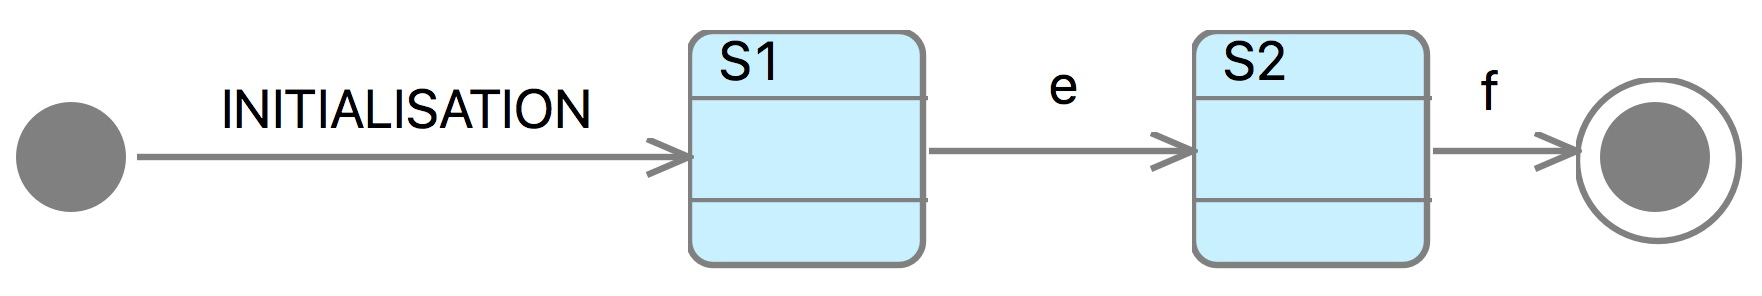
\includegraphics[width=0.6\textwidth]{figures/iumlb-SM}
% 	\caption{An example \UMLB state-machine}
% 	\label{fig:iumlb-sm}
% 	\vspace{-.5cm}
% \end{figure}

Each state is encoded as a boolean variable and the current state is indicated by one of the boolean variables being set to |TRUE|. 
An invariant ensures that only one state is set to |TRUE| at a time.
%The state-machine, is initialised by setting one state variable to |TRUE| and all others to |FALSE|.
Events change the values of state variables to move the |TRUE| value according to the transitions in the state-machine.  
% The \EventB translation%
% %
% \footnote{%
%   Here, $\mathrm{partition(S, T1, T2, \ldots)}$ means the set $S$ is partitioned into disjoint (sub-)sets $T1, T2, \ldots$.
% that cover $S$} 
% of the state-machine in Figure~\ref{fig:iumlb-sm} can be seen in Listing~\ref{lst:eventb-sm}.
% \UMLB also provides the option of an alternative translation with a single state variable ranging over an enumerated type of states, however, the boolean representation of each state is more natural for a user to reference in \SCXML guards and actions.
	
While the \UMLB translation deals with the basic data formalisation of state-machines it differs 
significantly from the semantics discussed in this manuscript. 
\UMLB adopts \EventB's simple guarded action semantics and does not have a concept of triggers and run-to-completion.
Here we make use of \UMLB's state-machine translation but provide a completely different semantic by generating a behaviour into the underlying \EventB events that are linked to the generated \UMLB transitions.
% \begin{lstlisting}[caption={Translation of the state-machine in Fig.~\ref{fig:iumlb-sm}},label={lst:eventb-sm}, language=Event-B, escapechar=|, frame=single]
% variables S1 S2
% invariants 
% 	TRUE !: {S1, S2} => partition({TRUE}, {S1}/\{TRUE}, {S2}/\{TRUE})
% events
%     INITIALISATION: begin S1, S2 := TRUE, FALSE end
%     e: when S1 = TRUE then S1, S2 ≔ FALSE, TRUE  end
%     f: when S2 = TRUE then S2 := FALSE end
% end
% \end{lstlisting}
%%% Local Variables:
%%% mode: latex
%%% TeX-master: "../main"
%%% End:
